
For the working mathematician, a basic application goes something like this.

The Fibonacci sequence $F_n$ ($n= 1, 2, \ldots$) is a \textit{strong divisibility sequence}, in that we have $\gcd(F_n, F_m) = F_{\gcd(n,m)}$; in particular, $F_m$ divides $F_n$ if $m \, | \, n$.  What about the special case $F_{3n}/F_n$?  And how could one possibly investigate this question using Gr\"obner bases?  It turns out that there is an identity:
\begin{equation}\label{F3n}
(F_{3n} - 5 F_n^3 - 3 F_n)(F_{3n} - 5 F_n^3 + 3 F_n) = 0,
\end{equation}
which explains explicitly this strong divisibility in this case.  How was such an identity obtained?  Here is the code:
\begin{M2}
\begin{verbatim}
i1:  R = QQ[z, x, y, t, MonomialOrder => Eliminate 2]
i2: I = ideal(x + y - z, (x*z - y^2)^2 - 1, t - z^3 - y^3 + x^3)
i3: toString groebnerBasis I
o3 = matrix {{25*y^6-10*y^3*t-9*y^2+t^2, z-x-y, ...
\end{verbatim}
\end{M2}  
\medskip
One can check that factoring the first polynomial in the list above gives (\ref{F3n}).  Bootstrapping this with extra equations, we can discover that:
\begin{equation}\label{F5n}
(F_{5n} - 25 F_n^5 - 25 F_n^3 - 5 F_n)(F_{5n} - 25 F_n^5 + 25 F_n^3 - 5 F_n) = 0,
\end{equation}
In fact, this more delicate analysis shows that $5F_n \, | \, F_{5n}$.  In turn, this incites conjectures and proofs.  This is an example of the promise of symbolic computation (with Gr\"obner bases) for the recreational mathematician, but there is more than this possible.

Consider the case of vertex 3-colorings of graphs.  Although exponential in the worst-case \cite[pp. 400]{yap2000fundamental}, Gr\"obner bases methods can be used to check or disprove conjectures in graph theory.  This was outlined theoretically in \cite{bayer1982division}, with success on a moderate-sized example \cite{hillar2008algebraic}, so-called Xu's conjecture \cite{shaoji1990size}, previously proved by other means and in much greater generality \cite{akbari2001kr}.

\begin{figure}
\begin{center}
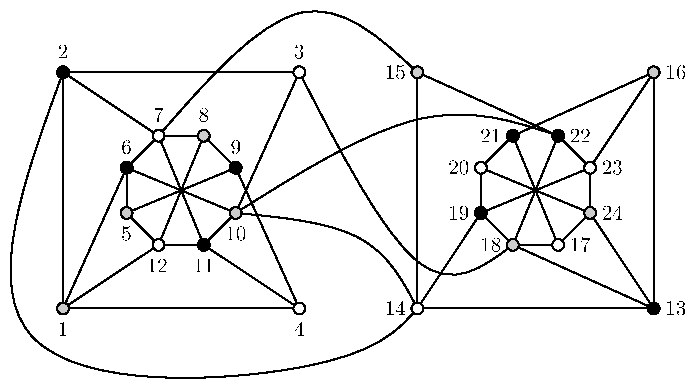
\includegraphics[width=.8 \linewidth]{akbarigraph.pdf}
\caption{Uniquely vertex 3-colorable graph without triangles: a counterexample \cite{akbari2001kr} to Xu's conjecture \cite{shaoji1990size}, which can be proved using Gr\"obner bases \cite{hillar2008algebraic}.}\label{graph}
\end{center}
\end{figure}



Groebner bases:

Drensky ``Grobner bases of ideals invariant under endomorphism".




Here we list the various applications of computation in rings with infinite numbers of indeterminates.  

\subsubsection{Group theory}

First studied in the context of group theory by Cohen in \cite{cohen1967laws}.

\subsubsection{Chemistry}

First appeared in algebraic chemistry \cite{} Ruch reference, and then attacked here \cite{aschenbrenner2007finite} and here Draisma \cite{Draisma08b}.

\subsubsection{Algebraic Statistics}

Diaconis Sturmfels \cite{diaconis1998algebraic}.

Independent set conjecture proved here \cite{hillar2012finite}, but early Japanese references \cite{}.

abelian tree models \cite{draisma2015finiteness}.

finiteness $k$-factor model chirality varieties \cite{Draisma08b}.

ideals of equivariant tree models \cite{draisma2009ideals}.

\subsubsection{Algebraic Geometry}

moduli space $n$ points in a line \cite{howard2009equations}.

length of Betti table goes to infinity: \cite{ein2015asymptotics}

and positivity of the the embedding line bundle grows: \cite{ein2012asymptotic}

also, more Draisma \cite{draisma2015plucker}.

\subsubsection{Topology}

Homological stability \cite{randal2013homological} and \cite{church2012homological}.


\subsubsection{Toric Algebra}



See \cite{Hillar13, hillar2016corrigendum} and \cite{draisma2013noetherianity}.  And recently \cite{KKL:equivariant-markov}.

\subsubsection{Tensor Geometry}

Here is a link to Draisma's work on this:  \cite{draisma2014bounded}.

\subsubsection{Category Theory and Asymptotic Algebra}

FI-algebras \cite{church2014fi, church2015fi}.  Asymptotic Hilbert series \cite{Nagel}, \cite{krone2016hilbert} and commutative algebra. 

General linear group replacing symmetric group \cite{}.

\subsubsection{Representation and category theory}

Noetherian property of infinite EI categorie \cite{gan2015noetherian}

\cite{putman2014representation}

grobner methods for representations of combinatorial categories: \cite{sam2016grobner}

GL-equivariant \cite{sam2016gl}









